\documentclass{llncs}

\usepackage[T1]{fontenc}
\usepackage{ifpdf}
\usepackage{url}
\usepackage{tabularx}
\ifpdf
\usepackage[pdftex]{graphicx}
\graphicspath{{figs/}}
\DeclareGraphicsExtensions{.pdf,.png,.jpg}
\else
\usepackage[dvips]{graphicx}

\graphicspath{{eps/}}
\DeclareGraphicsExtensions{.eps}
\fi
\usepackage{float}
%\usepackage[caption=false,font=footnotesize]{subfig}
\usepackage[font=footnotesize]{caption}
\usepackage{subcaption}
\captionsetup{compatibility=false}
\usepackage{setspace}
\usepackage{balance}
\hyphenation{op-tical net-works semi-conduc-tor}
\newcommand{\indentitem}{\setlength\itemindent{0pt}}
\usepackage{algorithmic}
\usepackage{algorithm}
\newcommand{\algorithmicinput}{\textbf{Input:}}
\newcommand{\INPUT}{\item[\algorithmicinput]}
\newcommand{\algorithmicoutput}{\textbf{Output:}}
\newcommand{\OUTPUT}{\item[\algorithmicoutput]}
\renewcommand{\algorithmicrequire}{\textbf{Pre Condition:}}
\renewcommand{\algorithmicensure}{\textbf{Post Condition:}}
\floatname{algorithm}{Procedure}
\usepackage{tikz}
\usetikzlibrary{matrix,arrows,circuits.ee,circuits.ee.IEC,shapes.geometric,shapes.misc}
\newcommand{\iap}{\textit{DREMS}}
\newcommand{\iapfull}{\textbf{D}istributed \textbf{RE}altime \textbf{M}anaged \textbf{S}ystem}% Algorithmic modifications
\newcommand{\ALOOP}[1]{\ALC@it\algorithmicloop\ #1%
  \begin{ALC@loop}}
\newcommand{\ENDALOOP}{\end{ALC@loop}\ALC@it\algorithmicendloop}
\renewcommand{\algorithmicrequire}{\textbf{Input:}}
\renewcommand{\algorithmicensure}{\textbf{Output:}}
\newcommand{\algorithmicbreak}{\textbf{break}}
\newcommand{\BREAK}{\STATE \algorithmicbreak}
\usepackage{color}

%\usepackage{url}
%\urldef{\mailsa}\path|{pkumar, dabhishe, gabor}@isis.vanderbilt.edu| 

\long\def\/*#1*/{}   

\newenvironment{noindlist}
 {\begin{list}{\labelitemi}{\leftmargin=0.1em \itemindent=0em \itemsep=0.3em}}
 {\end{list}}
\usepackage{multirow}
\begin{document}
\title{Colored Petri Net-based Modeling and Formal Analysis of Component-based Applications}

\author{Pranav Srinivas Kumar, Abhishek Dubey and Gabor Karsai}
\institute{Institute for Software Integrated Systems \\Department of Electrical Engineering and Computer Science\\
Vanderbilt University, Nashville, TN 37235, USA\\
{\bf \{pkumar, dabhishe, gabor\}@isis.vanderbilt.edu}}
\maketitle 
\vspace{-0.3in}

\begin{abstract}
Distributed Real-Time Embedded (DRE) Systems that address safety and mission-critical system requirements are applied in a variety of domains today. Complex, integrated systems like managed satellite clusters expose heterogeneous concerns such as strict timing requirements, complexity in system integration, deployment, and repair; and resilience to faults. Integrating appropriate modeling and analysis techniques into the design of such systems helps ensure predictable, dependable and safe operation upon deployment. This paper describes how we can model and analyze applications for these systems in order to verify system properties such as lack of deadline violations. Our approach is based on (1) formalizing the component operation scheduling using Colored Petri nets (CPN), (2) modeling the abstract temporal behavior of application components, and (3) integrating the business logic and the component operation scheduling models into a concrete CPN, which is then analyzed. This model-driven approach enables a verification-driven workflow wherein the application model can be refined and restructured before actual code development.
%
%component-based software applications i
%
%In this paper, we present a Colored Petri net-based approach to modeling and analysis of component-based software applications for enabling the verification of system properties such as lack of deadline violations. The approach is based on (1) formalizing the component operation scheduling using Colored Petri nets (CPN), (2) modeling the abstract temporal behavior of application components, and (3) integrating the business logic and the component operation scheduling models into a concrete CPN, which is then analyzed. This model-driven approach enables a verification-driven workflow wherein the application model can be refined and restructured before actual code development.
\end{abstract}

%\vspace{-0.2in}


\chapter{Introduction}
\label{chapter:introduction}

The decisive role of optimized and robust software in safety and mission-critical distributed real-time embedded (DRE) systems is becoming increasingly recognized. Embedded software is pertinent in a variety of heterogeneous domains e.g. avionics \cite{burke2010distributed}, automotive systems \cite{navet2008automotive}, locomotives \cite{zimmermann2003train}, and industrial control systems \cite{zoitl2008real}. The volume and complexity of such software grows everyday depending on an assortment of factors, including challenging system requirements e.g. resilience to hardware and software faults, remote deployment and repair. Deployment, the procedure for launching or reconfiguring software processes on embedded hardware, becomes extremely difficult if obtaining access to such devices is limited. Large scale deployment of embedded software, for this reason, has become considerably more arduous -- periodic peer reviews, numerous verification and certification methods are applied to maintain industry standards for safety, precision and reliability of embedded real-time software. Even still, software errors manifest in deployed systems; errors that can be extremely difficult to reproduce in a laboratory test environment. 

There exists a long list of real-world scenarios where errors in embedded software implementations has cost millions of dollars and human life. Between 1999 and 2010, at least 2,200 Toyota vehicles sold in the United States experienced unintended cases of rapid acceleration, causing nearly 900 accidents and over 100 deaths \cite{Cusumano:2011:RTD:1866739.1866750}. In 2010, Toyota recalled some 10 million vehicles, an extraordinary number given that the company sold only about seven million vehicles during that period. Toyota engineers described the problem as a disconnect in the vehicle's complex anti-lock brake system (ABS) that causes less than a one-second lag in its operation. With this delay, a vehicle going 60 mph will have traveled nearly another 90 feet before the brakes begin to take hold. Brakes in Toyota hybrids such as the Prius operate differently from brakes in most cars. In addition to the standard brakes, which use friction from pads pressed against rotors, the embedded software driving the electric motors help slow the vehicle. This process also generates electricity to recharge the batteries. This is a prime example of how timing errors in consumer-focused embedded software, spanning millions of lines of code, can have disastrous effects to everyday life. The Prius is Toyota's third best-selling model in the United States. The automaker recalled 2.3 million vehicles on January, 2011 because of problems with sticking gas pedals and later halted the sale of the eight models involved in the recall. Toyota's U.S. sales plunged 16 percent in January as a result, even as sales of other automakers rose.

To mitigate such software complexity, model-driven component-based software engineering (CBSE) and development \cite{beydeda2005model, heineman2001component, clemens1998component, simulink1993mathworks, autosar} has become an accepted practice. CBSE tackles escalated demands with respect to requirements engineering, high-level design, error detection, tool integration, verification and maintenance. The widespread use of component technologies in the market has made CBSE a focused field of research in the academic sectors. Applications are built by assembling together small, tested component building blocks that implement a set of services. These building blocks are typically built from UML \cite{UML} class diagrams, or imported from other projects/vendors and \emph{connected} together via exposed interfaces, providing a "black box" approach to software construction. This approach also treats software verification in a more modular fashion; the various software components can be verified individually and then composed together to derive a functional system. 

Remote embedded devices e.g. fractionated spacecraft \footnote{A fractionated spacecraft is a satellite architecture where the functional capabilities of a conventional monolithic spacecraft are distributed across multiple modules which interact through wireless network links.} following mission timetables and hosting distributed software applications expose several concerns including strict timing requirements, complexity in deployment, repair and integration; and resilience to faults, including mechanical failures like surface fractures, electrical failures such as single-event upsets, and manufacturing defects, and lastly software failures such as design defects and run-time faults. High-security and time-critical software applications hosted on such platforms run concurrently with all of the system-level mission management and fault recovery tasks that are periodically undertaken on the distributed nodes. Once deployed, it is often difficult to obtain a reliable period of low-level access to such remote systems for runtime debugging and evaluation. These types of DRE systems, therefore demand comprehensive design-time modeling and analysis methods to detect possible anomalies in system behavior, like the unacceptable response times in the advanced braking systems in vehicles. 

With the DARPA System F6 Project, our team has designed and prototyped a full information architecture called \emph{\textbf{D}istributed \textbf{RE}al-time \textbf{M}anaged \textbf{S}ystems} (DREMS) \cite{ISIS_F6_Aerospace:12,DREMS13Software} that addresses requirements for rapid component-based application development and deployment for fractionated spacecraft. The stack of developed software includes a  design-time model-driven development tool suite \cite{ISIS_F6_SFFMT:13}, and a component model \cite{ISIS_F6_ISORC:13} with precise execution semantics enabling robust and analyzable software designs. The minutiae of the DREMS architecture are described in Chapter \ref{chapter:DREMS}. The formal modeling and analysis methodology presented in this dissertation focuses on applications that rely on this foundational architecture. 

The principle behind design-time analysis here is to map the structural and behavioral specifications of the system under analysis into a formal domain for which analysis tools exist. The key is to use an appropriate model-based abstraction such that the mapping from one domain to another remains valid under successive refinements in system development such as code generation. The analysis must ensure that as long as the assumptions made about the system hold, the behavior of the system lies within the safe regions of operation. The results of this analysis will enable system refinement and re-design if required, before actual code development. 

\begin{figure}
	\centering
	\begin{subfigure}{.5\textwidth}
		\centering
		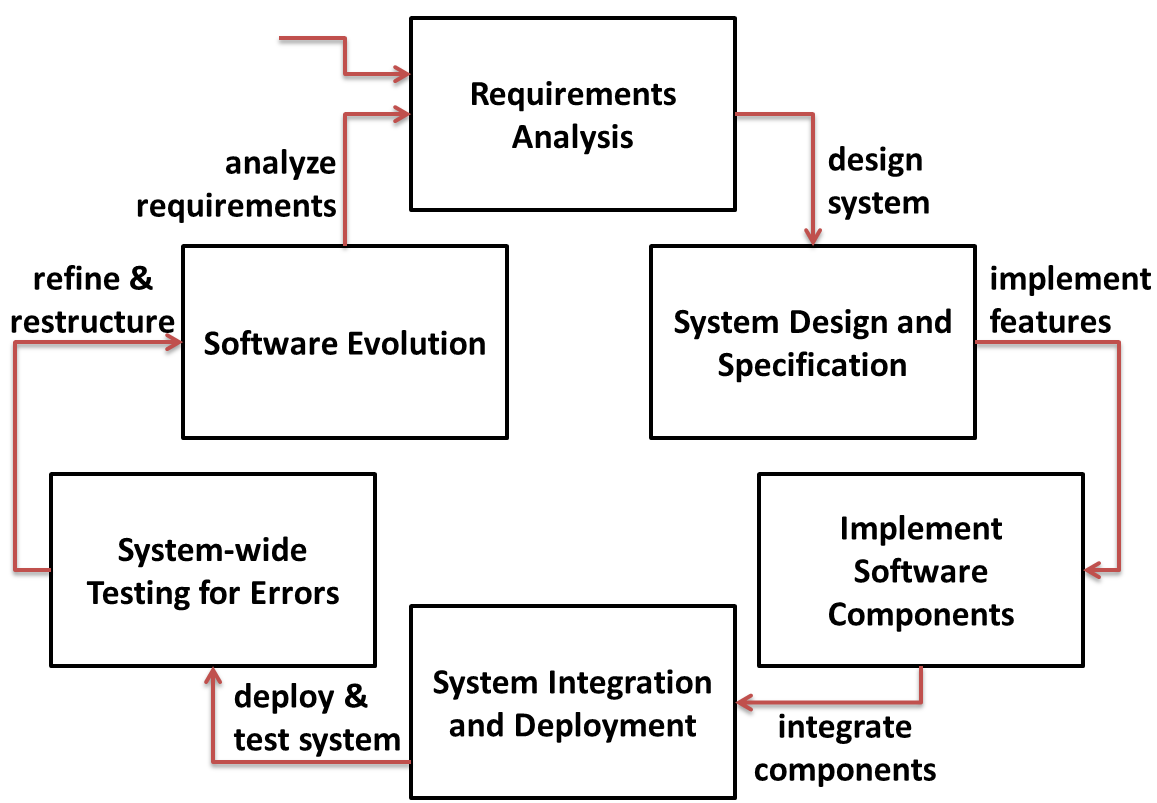
\includegraphics[width=0.9\linewidth]{sdlc}
		\caption{Industrial SDLC}
		\label{fig:sdlc}
	\end{subfigure}%
	\begin{subfigure}{.5\textwidth}
		\centering
		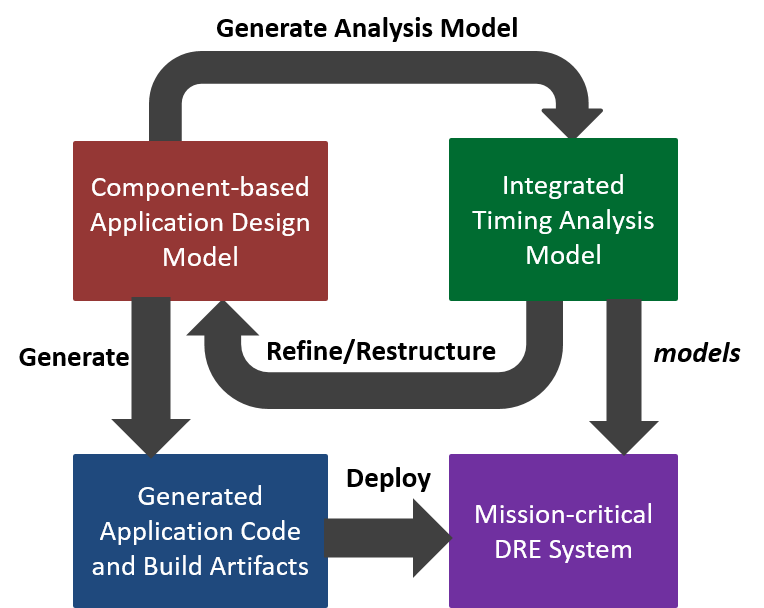
\includegraphics[width=\linewidth]{big_picture_2}
		\caption{DREMS Analysis-driven Workflow}
		\label{fig:big_picture}
	\end{subfigure}
	\caption{Embedded Software Development Lifecycle Comparison}
	\label{fig:test}
\end{figure}

Figure \ref{fig:sdlc} shows a \emph{spiral model} \cite{boehm1988spiral} of a typical industrial software/system development life cycle (SDLC). The five stages in this cycle include requirements analysis, software design, implementation, integration testing, and design evolution. Although the intricacies of each stage is hidden, the large majority of industrial software development follows this lifecycle. Embedded software development, especially for safety critical systems, does not lend itself well to this life cycle, mainly because the deliverable in such projects is usually not just a software package or a hardware platform but an amalgamation of both. Software development in fields like robotics, is tightly coupled with the hardware; assessment of software performance is sometimes dependent on and blocked by the hardware availability. Such blocking delays lead to inefficiencies in software evaluation and longer development times. It is also possible that design oversights could lead to poor timing performance e.g. long response times to critical events, that could damage the hardware in the process. Thus, the analysis presented in this work, supports and argues for a verification-driven workflow, as shown in Figure \ref{fig:big_picture}. The software evaluation is performed at design-time and as often as possible until the assembly is refined and optimized. Application developers use domain-specific modeling languages to structure large-scale component assemblies and modular code generation features to speed up software development efforts. Moreover, domain-specific properties such as interaction patterns, component execution code, and associated temporal properties such as worst-case execution times, deadlines etc. can be easily injected into such models. Using such application parameters in the \textit{design} model, a Colored Petri net-based (CPN) \cite{CPN} \textit{formal analysis model} is generated. The system behavior is both simulated and analyzed using a CPN execution engine, CPN Tools \cite{CPNTools}, and useful properties of the system are verified. By generating a bounded \emph{state space} of the system, the execution traces exhibited by the system are searched for property violations. Such system properties include the lack of deadlocks, deadline violations and worst-case trigger-to-response times. The goal of this analysis is to ensure that a component-based system: an assembly of tested component building blocks, meets the temporal specifications and requirements of the system.  

The results of this analysis will help improve the structure of the application, enabling safe deployment of dependable components that are known to operate within system specifications. Using CBSE also enables this restructuring process as the components are not tightly coupled software entities. So, when designing the integrated system, the analysis can be performed by assigning \emph{time budgets} to the discrete tasks in the execution. This enables timing analysis before implementation and also uses the time budgets as requirements for efficient code implementation. These budgets are often derived from some high-level requirements and appropriately distributed between the different components in the system. The analyzed system may not necessarily be complete, but instead be in a process of evolution. As the design progresses, the system requirements become concrete and the design is re-verified at each stage to ensure the consistency of all timing guarantees. 

The remainder of this dissertation is organized as follows. Chapter \ref{chapter:fundamentals} describes some fundamental concepts about distributed real-time systems, component-based software and some challenges in timing analysis. Chapter \ref{chapter:related-research} briefly describes general software testing and analysis methodologies, and summarizing related research in timing analysis and verification for distributed real-time embedded applications. Chapter \ref{chapter:DREMS} introduces the DREMS infrastructure and the Component Model used to experiment with and validate the timing analysis results. Chapter \ref{chapter:modeling} discusses the Colored Petri net-based timing analysis model devised for component-based DRE systems. Chapter \ref{chapter:analysis} describes the scope and efficiency of the analysis methods implemented with this CPN model. Chapter \ref{chapter:evaluation} evaluates this model with published results on analysis design, scalability and experimental validation. Finally, Chapter \ref{chapter:conclusion} concludes the dissertation, providing a summary of the detailed work and describing potential future work.
\vspace{-0.15in}

\section{Related Research}\label{sec:Related_Research}

\vspace{-0.1in}

In recent years, much of the proliferating work in the development of mission-critical distributed real-time systems addresses the need for Safety and Verification driven Engineering. Structural properties of the system are established using domain-specific modeling tools. Design models are transformed into relevant analysis models to study possible behaviors of the system and identify anomalies. When analyzing timing behavior, typically several exaggerated assumptions such as upper bounds on task execution times, service rates, maximum resource consumption etc are made. The results of system analysis using these assumptions are equally pessimistic. However, real-time systems with high criticality necessitate such assumptions to avoid the consequences of poor design. Predictability of system behavior is achieved by obtaining upper bounds on the system properties.   

Petri nets and their extensions have proven to be a powerful formalism for modeling and analyzing concurrent systems. System designs represented using a domain-specific modeling languages are often translated into Petri nets for formal analysis. High-level formalisms such as AADL models have been translated into Symmetric Nets for qualitative analysis \cite{kordon_sn} and Timed Petri nets \cite{kordon2009} to check for real-time properties such as deadline misses, buffer overflows etc. Similar to \cite{kordon2009}, our CPN-based analysis also makes use of observer places \cite{Alpern1989} that monitor the system behavior and look for real-time property violations and prompt completion of operations. However, \cite{kordon2009} only considers periodic threads in systems that are not preemptive. Our analysis covers a broader range of thread interaction patterns geared towards component-based applications operating on a hierarchical scheduling scheme requiring higher-level modeling concepts to capture component interaction in a distributed setup. 

In the context of component-based systems, for complete real-time analysis, significant information must be obtained about the component assembly, the interaction patterns and the temporal behavior of components. The real-time model of the system is composed of real-time models of its constituent parts, each with its own temporal behavior. Using abstract model descriptors, \cite{Lopez2006} describes a real-time model for component-based systems, including semantic and quantitative meta-data about component real-time behavior. Using the MAST transactional modeling methodology \cite{MAST1} and analysis tools in the MAST environment, schedulability checks and priority assignment automation are performed. Note here that for every real-time application, a separate and independent real-time analysis model is generated for each mode of operation and analyzed separately.

For classes of component-based systems whose component assembly and application structure change dynamically over time, design-time verification is observed to be insufficient. Incremental re-verification strategies \cite{johnson2013} have been applied to dynamic systems to augment traditional compositional verification by identifying the minimal set of components that require re-verification after dynamic changes. Since our approach considers design-time deployment plans that are static, our analysis does not consider dynamic changes to component assembly at run-time, but it will be subject of future work. 
\vspace{-0.15in}

\section{Background}
\label{sec:Background}

\vspace{-0.1in}

%\subsection{DREMS Components:}
%\label{sec:drems_component}

%\vspace{-0.05in}
\textbf{DREMS Components:}
Design and implementation of component-based software applications rests on the principle of assembly: \textit{Complex systems are built by composing re-useable interacting components}. Components contain functional, business-logic code that implements operations on state variables. Ports facilitate interactions between communicating components. A component-level message queue, with associated infrastructure code, controls the scheduling of operations of the individual components. Figure \ref{fig:drems_component} shows the basic DREMS component.

Each DREMS component supports four basic types of ports for interaction with other collaborating components: Facets, Receptacles, Publishers and Subscribers. A component's {\bf facet} is a unique interface that can be invoked either synchronously via remote method invocation (RMI) or asynchronously via asynchronous method invocation (AMI). A component's {\bf receptacle} specifies an interface required by the component in order to function correctly. Using its receptacle, a component can invoke operations on other components using either RMI or AMI. A {\bf publisher} port is a single point of data emission and a {\bf subscriber} port is a single point of data consumption. Communication between publishers and subscribers is contingent on the compatibility of their associated topics (i.e. data types). More details on this component model can be found in \cite{ISIS_F6_ISORC:13}.

%\vspace{-0.2in}

\begin{figure}[t]
	\centering
	\begin{subfigure}[b]{0.5\textwidth}
		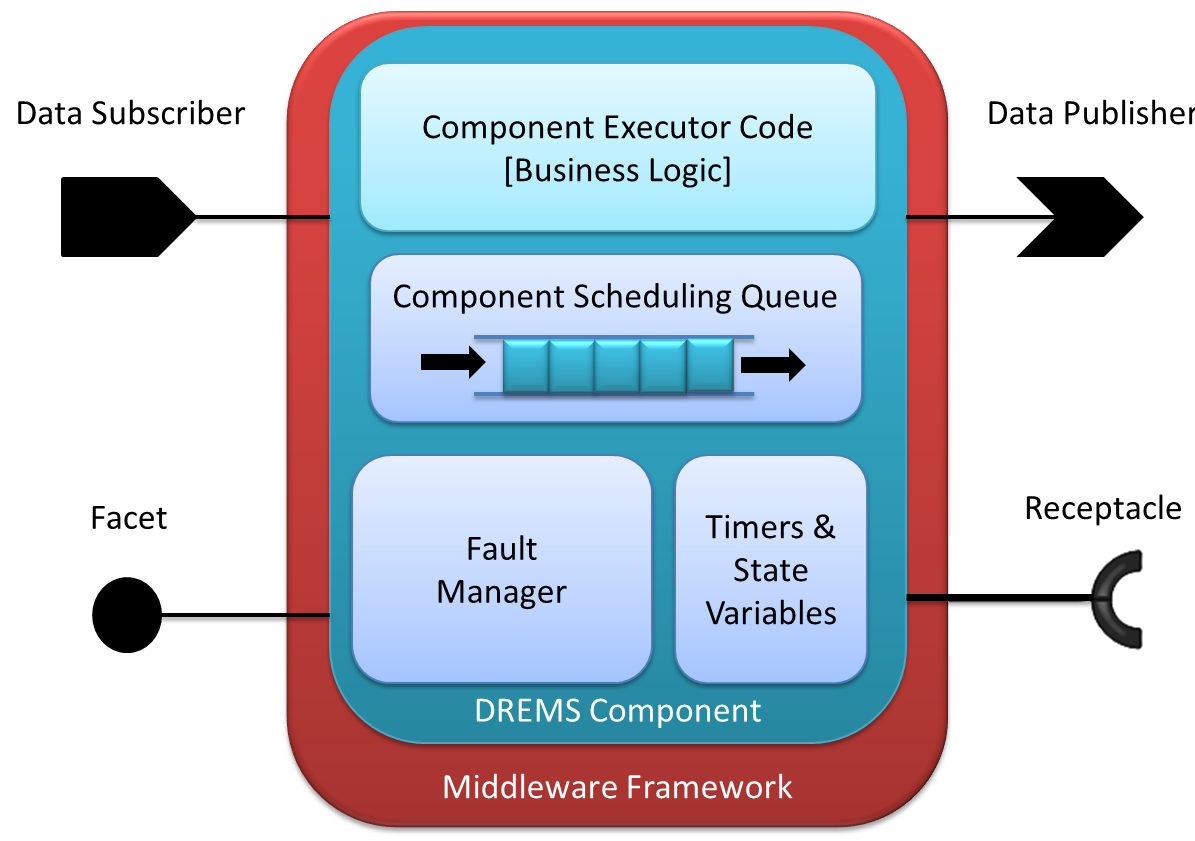
\includegraphics[width=\textwidth]{./figs/drems_component}
		\caption{DREMS Component}
		\label{fig:drems_component}
	\end{subfigure}%
	\begin{subfigure}[b]{0.5\textwidth}
		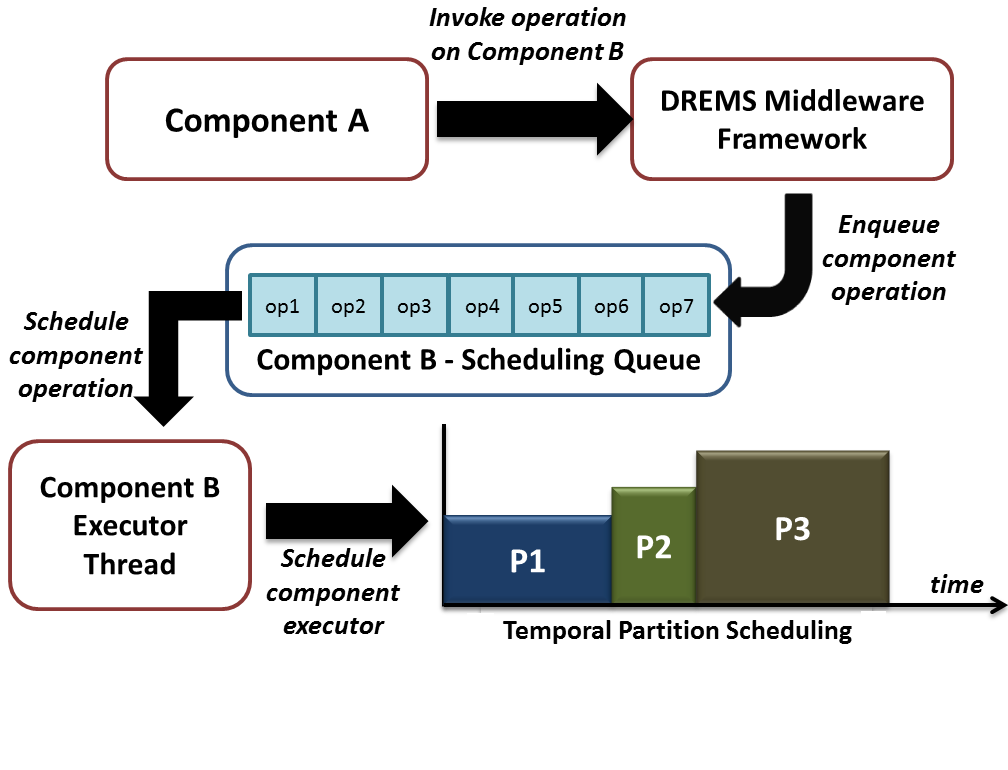
\includegraphics[width=\textwidth]{./figs/component_operations}
		\caption{Component Operation Scheduling}
		\label{fig:component_operations}
	\end{subfigure}
	\caption{DREMS Infrastructure}\label{fig:DI}
\vspace{-0.2in}
\end{figure}


\noindent
\textbf{Component Operation Scheduling:}
%\label{sec:component_operations}
%\vspace{-0.1in}
 An operation is an abstraction for the different tasks undertaken by a component. These tasks are implemented by the component's executor code written by the developer. As shown in Figure \ref{fig:component_operations}, in order to service interactions with the underlying framework and with other components, every component is associated with a message queue. This queue holds instances of operations ('messages') that are ready for execution and need to be serviced by the component. These operations service either interaction requests (seen on communication ports) or service requests (from the underlying framework). An example for the latter is the use of component timers that can periodically (or sporadically) activate an operation. Each operation is characterized by a priority and a deadline. The deadline here is the maximum acceptable time between the release of a component operation and the completion of that operation, measured starting from when the operation is enqueued onto the component's message queue.
To facilitate component behavior that is free of deadlocks and race conditions, the component's execution is handled by a single thread. This single-threaded execution helps avoid synchronization primitives such as internal lock variables that lead to tenuous code development.

The DREMS OS scheduler enforces an ARINC-653 ~\cite{ARINC-653} style temporal and spatial partition scheme in order to schedule components grouped into processes. Temporal partitions, as shown in Figure \ref{fig:component_operations}, are periodic fixed intervals of the processor time. Note that there are two levels of scheduling in DREMS: (1) Each component operation in the component-level is scheduled using a component-level scheduler, and (2) each component executor thread, on the system-level, is scheduled by the OS in one of the temporal partitions, granting a slice of the CPU's time to those threads.

\vspace{-0.2in}

\subsection{Colored Petri Nets}

\vspace{-0.1in}

Petri nets \cite{Murata1989} are a graphical modeling tool used for describing and analyzing a wide range of systems. A Petri net is a five-tuple $(P, T, A, W, M0)$ where P is a finite set of places, T is a finite set of transitions, A is a finite set of arcs between places and transitions, W is a function assigning weights to arcs, and M0 is the initial marking of the net. Places hold a discrete number of markings called tokens.  
A transition can legally fire when all of its input places have necessary number of tokens, and when fires it produces tokens for its output places. 

With Colored Petri nets (CPN) \cite{CPN}, tokens carry values of specific data types called colors. Transitions in CPN are enabled for firing only when valid colored tokens are present in all of the typed input places, and valid arc bindings are realized to produce the necessary colored tokens on the output places. The firing of transitions in CPN can check for and modify the data values of these colored tokens. Furthermore, large and complex models can be constructed by composing smaller sub-models as CPN allows for hierarchical description. This extended paradigm can more easily model and analyze systems with typed parameters. 

\vspace{-0.2in}

\section{Problem Statement}
\label{sec:Problem_Statement}

\vspace{-0.1in}
Consider a set of mixed-criticality component-based applications that are distributed and deployed across a cluster of embedded computing nodes. Each component has a set of interfaces that it exposes to other components and to the underlying framework. Once deployed, each component works by executing operations placed on its component message queue. Each component is associated with a single executor thread that handles these operation requests. These executor threads are scheduled in conjunction with a known set of highly critical system threads and low priority best-effort threads. Furthermore, the application threads are also subject to a temporally partitioned scheduling scheme. System assumptions include (1) knowledge of the sequence of computational steps of known duration that are executed inside each component operation, (2) knowledge of the worst-case estimated time taken by each computational step, and (3) the estimated worst-case time taken to initiate a remote function call and to process the response, accounting for network-level delays. Using this knowledge about the system, the problem here is to ensure that the temporal behavior of all the application components lies within the bounds laid out by the system specifications. Ideally, this is achieved by verifying such system properties as lack of deadline violations for component operations. For scenarios where the system design isn't complete, e.g. application thread priorities are unknown, the paper describes the utility of an approach to identifying the subset of system behaviors that satisfy timing requirements and provide useful information to designers, e.g. partial thread execution orders. 

\vspace{-0.2in}   

\section{Colored Petri net-based Modeling}
\label{sec:CPN_Modeling}

\vspace{-0.1in}

This section briefly describes how CPN can be used to build an extensible, scalable analysis model for component-based software applications. To edit, simulate and analyze this model, we use the CPN Tools \cite{CPNTools} tool suite. 

The CPN model captures the behavioral semantics of our component model described in \cite{ISIS_F6_ISORC:13}, using knowledge of several factors that resolve the deployment of the component-based application. These factors include the following system properties: (1) configuration of temporal partition scheduling on each node of the distributed system, (2) location of each component being deployed (which temporal partition and which computing node) (3) properties of the component executor threads (thread priority), (4) properties of timers (period and offset), and (5) component interactions and assembly (i.e. the 'wiring'). 

%\vspace{-0.2in}
\begin{figure}[t]
	\centering
	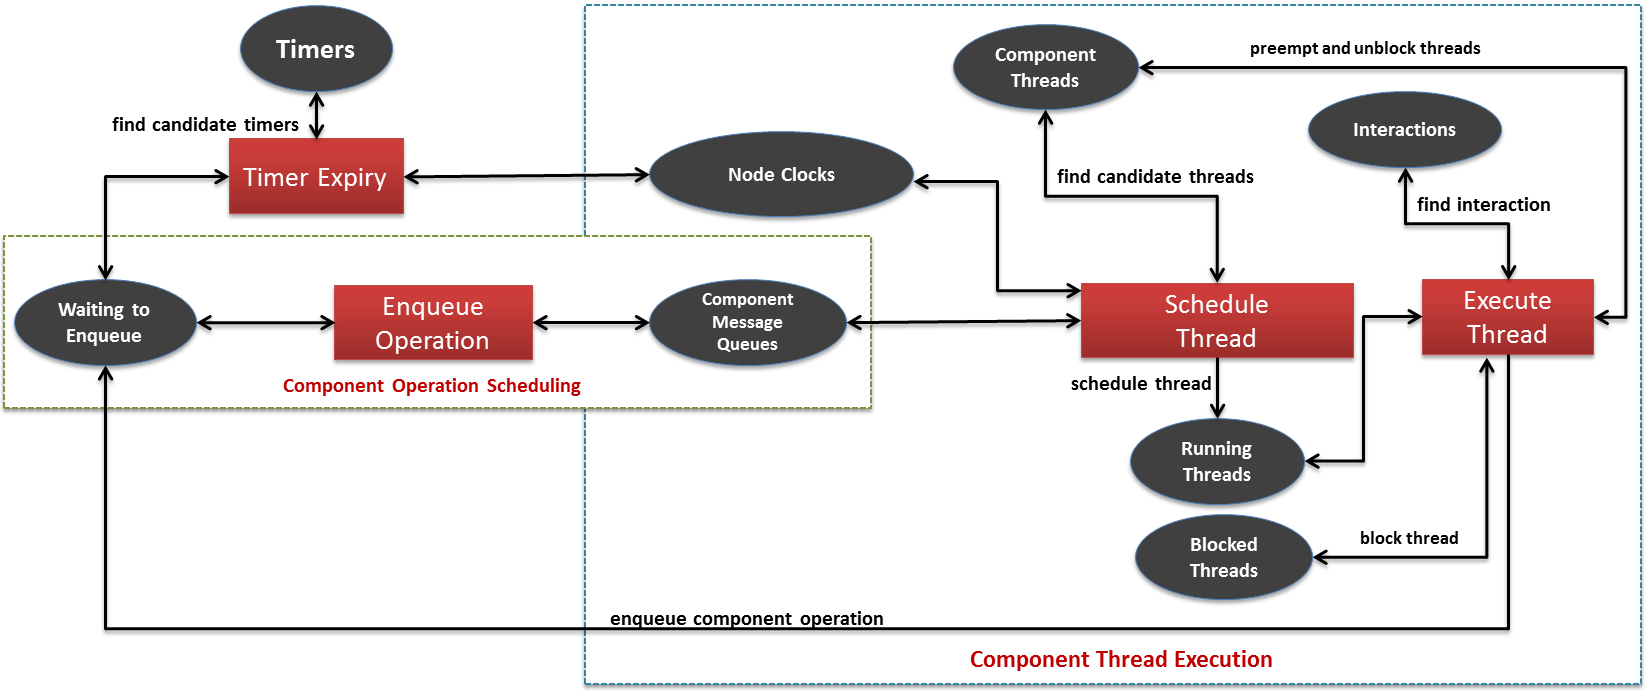
\includegraphics[width=\textwidth]{./figs/cpn_model}
	\caption{Hierarchical CPN Analysis Model}
	\label{fig:cpn_model}
	\vspace{-0.1in}
\end{figure}
%\vspace{-0.1in}

Figure \ref{fig:cpn_model} shows a top-level structure of the CPN-based analysis model. The place \emph{Component Threads} holds a token with a list of all executor threads responsible for component interactions. This list is maintained based on thread priorities on each node so that the highest priority ready thread is always chosen first by the OS scheduler. \emph{Timers} maintains a list of all infrastructural timers in the application. All timer expiries at a specific clock value\footnote{The clock values are integers.} are handled by the transition \emph{Timer Expiry}. A timer can be used in our component model to trigger the execution of a component operation. DREMS components are dormant by default.  Once initialized, a component executor is not eligible to run until there is an operation added to the component message queue. To start a sequence of component interactions, periodic or sporadic timers can be used to trigger an operation of a component.

If a timer triggers a component execution, this component is identified as a candidate for scheduling by \emph{Schedule Thread}. This transition always schedules the highest priority thread that is ready to execute in the active partition on each node. If two threads of equal priority are eligible, the scheduler picks one at random and maintains a round-robin scheduling scheme. If the highest priority thread is not already servicing an operation request, the highest priority operation from its message queue is dequeued and scheduled for execution.

The \emph{Component Message Queues} place is a list that manages the message queues of all components across all nodes. Every time a component thread executes an operation, the completion of this operation could trigger another component into execution. For instance - the completion of an RMI query on a client component triggers a server-side RMI operation that this server will have to execute. Such interactions are derived from the modeling tools and appropriate tokens are generated in place \emph{Interactions}. When executing component threads, \emph{Execute Thread} checks to see if the execution has any effect on the running thread or on other threads. Therefore, when the client thread completes an RMI query, this thread is moved to \emph{Blocked Threads} and a server RMI operation is placed in \emph{Waiting to Enqueue}. Later, when the server thread is scheduled, the client is unblocked appropriately.






\vspace{-0.2in}

\section{State Space Analysis}
\label{sec:State_Space_Analysis}

%\vspace{-0.4in}

\begin{figure}[t]
	\centering
	\begin{subfigure}[b]{0.5\textwidth}
		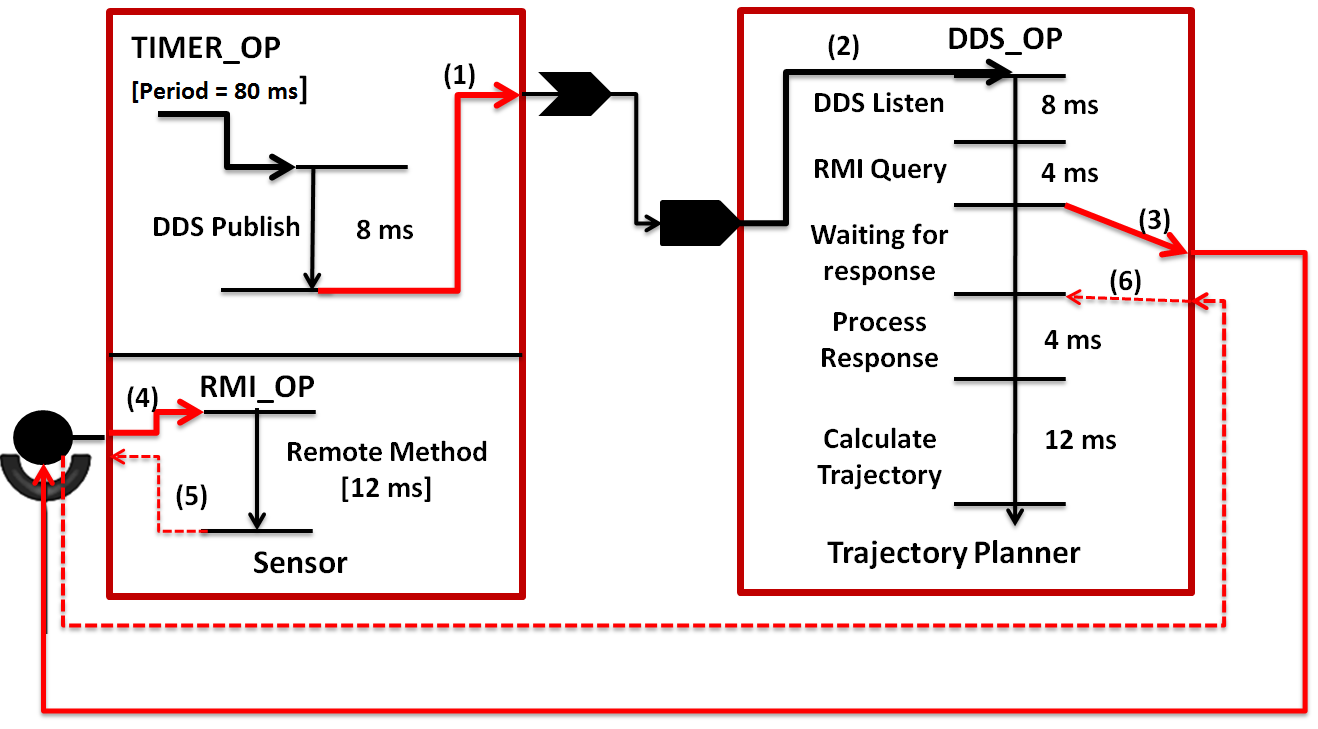
\includegraphics[width=\textwidth]{./figs/tpa}
		\caption{Component Assembly}
		\label{fig:tpa}
	\end{subfigure}%
	\begin{subfigure}[b]{0.5\textwidth}
		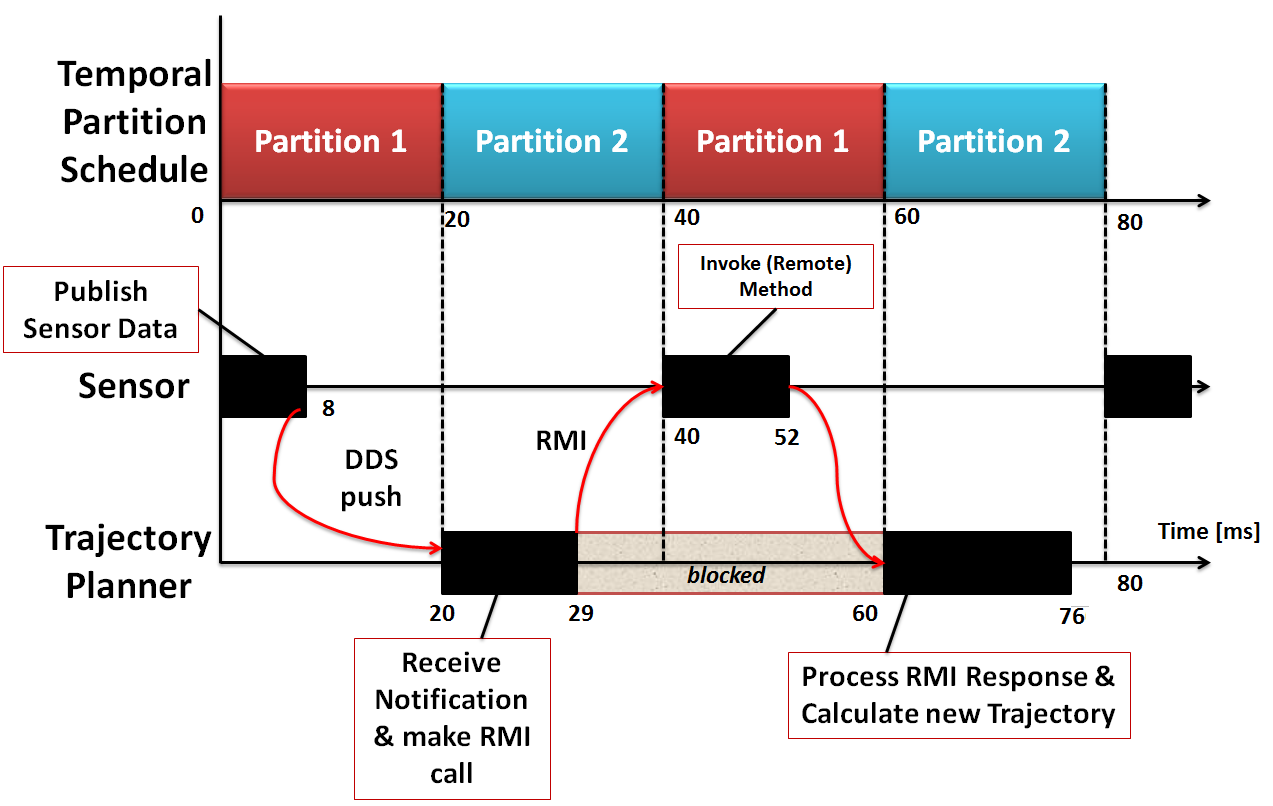
\includegraphics[width=\textwidth]{./figs/tpa_td}
		\caption{Timing Diagram}
		\label{fig:tpa_td}
	\end{subfigure}
	\caption{Trajectory Planning Application}\label{fig:TPA}
%\vspace{-0.2in}
\end{figure}



Given a CPN model (that was generated from a component architecture and deployment model), a state-space of the system can be constructed using the semantics of CPN. This state space is infinite, however, in practice, it is often sufficient to consider some finite subset, starting from a initial state up to a few hyperperiods of the partition scheduler. In order to describe the utility of state space analysis, we consider a simple trajectory planning application (TPA). The component assembly for this application is shown in Figure \ref{fig:tpa}. A Sensor component periodically publishes on a trigger topic, notifying the Trajectory Planner of the existence of new sensor data. Once the notification is received, the Trajectory Planner makes an RMI call to retrieve the data structure of sensor values, using which the satellite trajectory is updated. The sequence of steps in each of these operations is referred to as the business logic of the operation. This business logic is modeled using a textual language in the modeling tools, in which the designer specifies the macro execution steps in a component operation along with worst-case estimated time taken on each step. Figure \ref{fig:tpa_td} shows the expected timing diagram. 

The analyzable states of this system are observed in the markings of the various CPN places in the model. Using the built-in state space analysis in \textit{CPN Tools} a bounded state space of the system is generated. Using both standard and user-defined queries, this state space is searched to check system properties like lack deadline violations and deadlocks, bounds on response times etc.

\vspace{-0.1in}

\subsubsection{Deadline Violation Detection:}

Each time a component operation is scheduled, the clock value of the node is recorded as the "start time" of the operation. If this operation is incomplete when the clock reaches the operation's deadline, a deadline violation is detected. Using the \emph{SearchNodes} function in CPN Tools, the deadline violations on any component operation can be identified by observing all component operations each time the node-specific clock progresses. In Figure \ref{fig:tpa_td}, the \emph{DDS\_OP} on the Trajectory Planner takes 56 ms to complete, measured from when the operation was enqueued and marked as ready. If the deadline of this operation is set to 50 ms, a state space search would reveal a deadline violation when the clock reaches 51 ms.

\vspace{-0.1in}

\subsubsection{Worst-case Trigger-to-Response Time Calculation:}

For a known trigger operation and desired response operation, the worst-case trigger-to-response time can also be calculated from the generated state space. Using the names of the trigger and response operations, a state space node that presents the earliest completion of the trigger operation and the latest completion of the response operation within the set period is identified. In the Trajectory Planning application, considering the \emph{TIMER\_OP} to be the trigger and the trajectory planning \emph{DDS\_OP} to be the response, the worst-case response time is found to be 68 ms (Trigger completes earliest at 8 ms and response completes latest at 76 ms). 

\vspace{-0.1in}

\subsubsection{Partial Thread Execution Order Generation:}

In development scenarios where an application developer is aware of the operation-specific timing requirements but not thread priorities, the analysis is capable of identifying partial thread execution orders that satisfy the requirements. If all unknown thread priorities are set to a common value, the generated partial state space will then encapsulate the set of non-deterministic thread execution orders that arise from the scheduling. Using timing requirements of the form - \emph{Once Operation A on Component A on Node A completes, Operation B on Component B on Node B must complete within 150 ms}, a state space node satisfying this requirement can be identified by querying the generated state space. A backtrace from this node enables assigning thread priorities to ensure the satisfaction of the timing requirement.

\vspace{-0.15in}
\subsubsection{Scalability Testing:}
\label{sec:Scalability_Testing}

The size of the generated state space is dependent on the amount of concurrency in the behavior. If all the executing threads had unique priorities, the thread execution order is a constant as the scheduling is priority-based. However, for large systems with groups of applications and increased concurrency, an equally large state space is required to observe the tree of possible thread executions and operational behaviors. This analysis model has been identified to scale well for medium-sized applications, tested up to 100 components distributed on up to 5 computing nodes. Table \ref{table:scalability} summarizes these results.

\vspace{-0.1in}

\section{Analysis Model Generation}
\label{sec:Model_Generation}

\vspace{-0.1in}

As mentioned in Section \ref{sec:CPN_Modeling}, the control flow and timing details of component operations are directly integrated into the design-time modeling framework. Using the formal domain-specific model of the system, the configuration of the partition scheduling and component assembly are derived and translated into meaningful CPN tokens. The business logic of each component operation is expressed using a textual language with one attribute per interaction per instance of each component being deployed. Model interpreters parse through this complete design model, instantiating CPN model templates and combining these instances to generate a single integrated .cpn file to analyze the entire system.

%\vspace{-0.4in}

\begin{table}[t]
	\caption{Scalability Results}
	\label{table:scalability}
	\begin{center}
		\begin{tabular}{ | c | p{1cm} | p{1.7cm} | p{1.7cm} | p{1.4cm} | p{1.3cm} | p{1.7cm} |}
			\hline
			Scenario & Nodes & Partitions / Node & Threads / \mbox{Partition} & Hyper-periods & State Space & Generation Time\\ \hline
			TPA & \multicolumn{1}{|c|}{5} & \multicolumn{1}{|c|}{2} & \multicolumn{1}{|c|}{1} & \multicolumn{1}{|c|}{10} & \multicolumn{1}{|c|}{180} & \multicolumn{1}{|c|}{0.981s}\\ \hline
			Sample2 & \multicolumn{1}{|c|}{2} & \multicolumn{1}{|c|}{5} & \multicolumn{1}{|c|}{5} & \multicolumn{1}{|c|}{10} & \multicolumn{1}{|c|}{124,469} & \multicolumn{1}{|c|}{14.1m} \\ \hline
			Sample3 & \multicolumn{1}{|c|}{5} & \multicolumn{1}{|c|}{5} & \multicolumn{1}{|c|}{4} & \multicolumn{1}{|c|}{10} & \multicolumn{1}{|c|}{485,552} & \multicolumn{1}{|c|}{36.5m} \\ \hline			
		\end{tabular}
	\end{center}
\vspace{-0.2in}
\end{table}

%\vspace{-0.4in}

%\vspace{-0.2in}

\section{Future Work}
\label{sec:Future_Work}

\vspace{-0.1in}
 
In order to generalize this analysis model and provide flexibility, one possible extension to this approach is to cater to other commonly used scheduling schemes, such as EDF, for component operation scheduling; and novel interaction patterns (e.g. reliable broadcast). Also, the current analysis approach inherits the benefits and the drawbacks of using pessimistic estimates for execution times. Another possible extension to this approach would be to provide a stochastic schedulability analysis allowing for a trade-off between reliability and cost of resources required by the system. 

\vspace{-0.2in}

\section{Conclusions}
\label{sec:Conclusions}

\vspace{-0.1in}

Distributed real-time systems operating in dynamic environments, and running mission-critical applications face strict timing requirements to operate safely. %To reduce the development and integration complexity for such systems, component-based design models are being increasingly used. Appropriate analysis models are required to study the structural and behavioral complexity in such designs. 
This paper presents a Colored Petri Net-based approach to capture the architecture and temporal behavior of such applications for both qualitative and quantitative schedulability analysis. This analysis model includes a compact, scalable representation of high-level design, accounting for the dynamics of real-time thread execution while exploiting knowledge of component execution code. Exhaustive state space search enables verification and validation of useful and necessary system properties, reducing development costs and increasing reliability for such time-critical systems. 

\vspace{-0.2in}

\section*{Acknowledgments}\label{sec:Acknowledgments}

\vspace{-0.1in}

The DARPA System F6 Program and the National
Science Foundation (CNS-1035655) supported
this work. Any opinions, findings, and conclusions or recommendations expressed
in this material are those of the authors and do not reflect the views of
DARPA or NSF. 

\vspace{-0.2in}

\bibliographystyle{splncs}
\bibliography{bibliography}

\end{document}